{ %section3_3
	\subsection{Технология OpenMP}
	\Large\par\textbf{Краткая характеристика технологии.} Первая версия стандарта OpenMP появилась в 1997 году при поддержке крупнейших IT-компаний мира (Intel, IBM, AMD, HP, Nvidia и др.). Целью нового стандарта было предложить кроссплатформенный инструмент для распараллеливания, который был бы более высокоуровневый, чем API управления потоками, предлагаемые операционной системой. На данный момент OpenMP стандартизована для трёх языков программирования: С, С++ и Фортран.
	\par\textbf{Поддержка компиляторами.} Абсолютное большинство существующих современных компиляторов С/С++ поддерживают OpenMP версии 2.0 (например, как gcc, так и Visual Studio). Однако лишь немногие компиляторы поддерживают более новую версию OpenMP 4.0, поэтому далее при изложении материала будет в качестве "общего знаменателя"\verb+ +использоваться технология OpenMP 2.0.
	\par OpenMP определяет набор директив препроцессору, которые дают указание компилятору заменить следующий за ними исходный код на его параллельную версию с помощью доступных компилятору средств, например с помощью POSIX Threads в Linux или Windows Threads в операционных системах Microsoft. Для корректной трансляции директив необходимо при компиляции указать специальный ключ, значение которого зависит от компилятора (примеры приведены в таблице~\ref{compilerOpenMP:table}).
	\begin{table}[H]
		\Large
		\caption{Ключи компиляторов для запуска OpenMP}
		\label{compilerOpenMP:table}
		\begin{center}
			\begin{tabular}{|c|c|}
				\hline
				\textbf{Название компилятора} & \specialcell{\textbf{Ключ компилятору для включения} \\  \textbf{OpenMP}} \\
				\hline
				Gcc & -fopenmp \\
				\hline
				icc (Intel C/C++ compiler) & -openmp \\
				\hline
				Sun C/C++ compiler & -xopenmp \\
				\hline
				Visual Studio C/C++ compiler & /openmp \\
				\hline
				PGI (Nvidia C/C++ compiler) & -mp \\
				\hline
			\end{tabular}
		\end{center}
	\end{table}
	\parПомимо препроцессорных директив, OpenMP определяет набор библиотечных функций, для вызова которых в исходном коде потребуется подключить заголовочный файл OpenMP:
	\begin{figure}[H]
		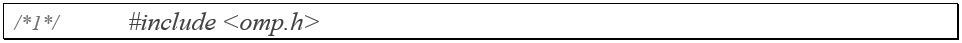
\includegraphics[width=1\linewidth]{includeOpenMP}
	\end{figure}
	\par\textbf{Отличительные особенности.} Среди прочих технологий распараллеливания OpenMP выделяется следующими важными и характеристиками:
	\begin{itemize}
		\itemИнкрементное распараллеливание.
		\itemОбратная совместимость.
		\itemВысокий уровень абстракций.
		\itemНизкий коэффициент трансформации.
		\itemПоддержка крупнейшими  IT-гигантами. 
		\itemАвтоматическое масштабирование.
	\end{itemize}
	\par\textit{Инкрементное распараллеливание.}  OpenMP позволяет распараллеливать существующую последовательную программу в виде  небольших итераций-правок, на каждой из которых будет достигаться всё больший коэффициент распараллеленности программы. Эта особенность является уникальной, т.к. большинство других технологий предполагают существенное изменение структуры распараллеливаемой программы уже на первом этапе процесса распараллеливания, при этом первая работоспособная параллельная версия программы появляется после длительного процесса отладки и программирования новых компонентов, которые неизбежно добавляются при распараллеливании. OpenMP лишён этого недостатка.
	\par\textit{Обратная совместимость.} Большинство программных технологий развиваются с обеспечением обратной совместимости (backward compatibility), когда более новая версия программы поддерживает работоспособность старых файлов. Термин \textit{"прямая совместимость"} (forward compatibility) имеет противоположный смысл: файлы, созданные в программе новой версии, остаются работоспособными при использовании старой версии программы. В случае OpenMP это проявляется в том, что распараллеленная программа будет корректно скомпилирована в однопоточном режиме даже на старом компиляторе, который не поддерживает OpenMP. Важно отметить, что прямая совместимость обеспечивается, если при распараллеливании не используются библиотечные функции OpenMP, а присутствуют только препроцессорные директивы. При наличии библиотечных функций для обеспечения обратной совместимости потребуется написать функции-заглушки в файле "omp.h" (лишь немногие компиляторы умеют генерировать эти заглушки при использовании специального ключа).
	\par\textit{Высокий уровень абстракций.} Одна единственная препроцессораня директива OpenMP после обработки компилятором приводит к существенной трансформации исходной программы с добавлением большого количества новой логики, отвечающей за определение доступного в системе количества процессоров, за запуск и уничтожение потоков, за распределение работы между потоками и т.п. Все эти операции OpenMP берёт на себя,  взамен программист получает набор очень высокоуровневых инструментов распараллеливания. У высокоуровневых языков есть и традиционная тёмная сторона: в OpenMP отсутствует возможность изменить некоторую внутренние детали работы с потоками (например, нельзя установить аффинность  потоков или уменьшить накладные расходы на создание/удаление потоков).
	\par\textit{Низкий коэффициент параллельной трансформации (КПТ).} При распараллеливании существующей последовательной программы приходится вносить в неё достаточно большое количество изменений. Пусть КПТ – это отношение строк нового программного кода, который добавился в результате распараллеливания, к общему количеству строк кода в программе. В OpenMP КПТ обычно существенно ниже, чем у большинства других технологий распараллеливания. Это объясняется высоким уровнем абстракции языка OpenMP (см. предыдущий пункт). 
	\par\textit{Поддержка крупнейшими  IT-гигантами.} Уже при разработке\\ OpenMP о его поддержке заявили крупнейшие игроки IT-мира. Это обеспечило не только высокое качество разработки стандарта, но и наличие готовых реализаций стандарта в популярных компиляторах. Несмотря на прошедшие два десятка лет OpenMP не растерял приверженцев и поддержка новейших версий OpenMP с достаточно малой задержкой появляется в компиляторах. Например, при текущей версии стандарта OpenMP 4.5 наиболее популярные компиляторы уже поддерживают версию OpenMP 4.0. Исключением является только фирма Microsoft. Их компилятор вот уже несколько версий неизменно поддерживает только \\OpenMP 2.0. 
	\par\textit{Автоматическое масштабирование.}  Низкоуровневые технологии распараллеливания (POSIX Threads, OpenCL) предлагают программисту вручную управлять количеством создаваемых потоков при выполнении параллельной работы. Это обеспечивает возможность гибко управлять и настраивать процесс создания потоков в зависимости от количества доступных системе процессоров (ядер), но при этом требует от программиста большой количества неавтоматизируемой работы. В OpenMP управление масштабированием происходит в автоматическом режиме, т.е. OpenMP сам запрашивает у операционной системы количество доступных процессоров и выбирает количество создаваемых потоков. Но при необходимости OpenMP оставляет возможность устанавливать требуемое количество потоков вручную.
	\par\textbf{Примеры OpenMP-программ.}
}